\documentclass[12pt,a4paper]{report}
\usepackage[utf8]{inputenc}
\usepackage{graphicx}
\usepackage{amsmath}
\usepackage{amssymb}
\usepackage{hyperref}
\usepackage{listings}
\usepackage{caption}
\usepackage{subcaption}
\usepackage{tocloft}
\usepackage{titlesec}
\usepackage[utf8]{inputenc}
\usepackage{hyperref}
\usepackage{url}
\usepackage[numbers,super]{natbib}
\usepackage{svg}

\renewcommand{\contentsname}{Cuprins}
\renewcommand{\bibname}{Bibliografie}

\titleformat{\chapter}[hang]
  {\normalfont\huge\bfseries}{\thechapter.}{1em}{}

\begin{document}

\begin{titlepage}
    \centering
    \vspace*{1cm}
    
    \Huge
    \textbf{Sistem Automat de Clasificare Malware Android}
    
    \vspace{0.5cm}
    \LARGE
    Lucrare de Licență
    
    \vspace{1.5cm}
    
    \textbf{Crețu Vlad-Sebastian}
    
    \vfill
    
    \Large
    Coordonator: Dr. Ing. Aciu Răzvan
    
    \vspace{0.8cm}
    
    % 
\includegraphics[width=0.4\textwidth]{university_logo.png}
    
    Universitatea Politehnica Timișoara\\
    Facultatea de Automatică și Calculatoare\\
    2024
    
\end{titlepage}

\tableofcontents
% \listoffigures
% \listoftables
% \lstlistoflistings

% \chapter*{Lista Abrevierilor}
% \addcontentsline{toc}{chapter}{Lista Abrevierilor}
% \begin{tabular}{ll}
%     API & Application Programming Interface \\
%     ML & Machine Learning \\
%     AV & Antivirus \\
% \end{tabular}

\chapter{Introducere}
\section{Context}
În prezent, sistemul de operare Android domină piața globală a dispozitivelor mobile, 
având o cotă de piață de peste 70\% din totalul dispozitivelor vândute \cite{stat-counter}. 
Numărul aplicațiilor Android disponibile pe Google Play, cel mai popular magazin online 
pentru acest sistem, a ajuns la 3.718 milioane în 2023, cu o predicție de 4.200 milioane
până în 2025 \cite{number-of-google-play-store-apps}. Această creștere va duce la 
necesitatea unui sistem scalabil capabil să proceseze și să analizeze zilnic cantități 
enorme de aplicații, pentru a asigura securitatea și confidențialitatea utilizatorilor platformei.
\section{Motivație}
Studiile disponibile se concentrează pe îmbunătățirea acurateței algoritmilor 
de predicție automată a malware-ului, lăsând preprocesarea datelor pe un plan secundar. 
Puține cercetări abordează în mod exhaustiv dezvoltarea unui sistem cap-coadă care să fie
atât eficient, cât și scalabil. În contextul unei creșteri a numărului de aplicații 
Android și a diversificării metodelor de atac, este esențial să se dezvolte soluții integrate 
care să includă atât preprocesarea datelor, cât și analiza și clasificarea acestora. 
Această lucrare își propune să umple acest gol, oferind un sistem complet care să poată 
preprocesa eficient datele, să le analizeze și să le clasifice automat pentru a 
evita atacurile malware.
\section{Obiective}
Lucrarea se concentrează pe dezvoltarea următoarelor obiective:
\begin{enumerate}
    \item Dezvoltarea unui sistem automat de clasificare multi-label a fișierelor APK\cite{apk-file-format-wiki} folosind 3 componente principale:
    \begin{itemize}
        \item Modul de preprocesare a datelor realizat folosind limbajul de programare Rust\cite{rustlang}, care se ocupă de extragerea permisiunilor și secvenței de cod din fișierele APK.
        \item Model de clasificare bazat pe algoritmi de învățare automată realizat folosind librăria Tensorflow\cite{tensorflow}, care va clasifica fișierele APK în una din 5 categorii: \textit{Adware, Banking, Benign, Riskware, SMS}.
        \item REST API realizat folosind framework-ul axum\cite{axum-framework} care va oferi o interfață programatică pentru a trimite fișiere APK spre clasificare și a primi rezultatele.
    \end{itemize}
    Vizualizarea predicțiilor se va face printr-o interfață web realizată folosind framework-ul React\cite{react}.
    \item Afișarea rezultatelor experimentale și a statisticilor relevante pentru a evalua performanța sistemului.
\end{enumerate}


\chapter{Analiza stadiului actual în domeniul problemei}
\section{Clasificare malware}
\section{Metode actuale de detectare}

\chapter{Fundamentare teoretică}

\section{Sistemul Android}
Android este un sistem de operare open source complet cu cod sursă personalizabil 
care poate fi portat pe aproape orice dispozitiv, și cu documentație publică disponibilă 
pentru toată lumea la \textit{source.android.com} pentru dispozitive mobile, condus de Google\cite{android-source}.
Platforma Open System Android (AOSP) este un cod sursă Android disponibil public și modificabil. 
Oricine poate descărca și modifica AOSP pentru dispozitivul său. 
AOSP oferă o implementare completă și funcțională a platformei mobile Android care constituie următoarea stivă de software\cite{android-architecture} (Figura \ref{fig:android_stack}):
\begin{enumerate}
    \item \textbf{API-ul Android} - API de nivel înalt public pentru dezvoltarea aplicațiilor third-party
    \item \textbf{Android Framework} - Un set de classe și interfețe Java precompilate care oferă funcționalități de bază pentru dezvoltarea aplicațiilor.
    O parte din framework este accesibilă prin Android API, pe când cealaltă este accesibilă doar prin API-ul sistemului.
    \item \textbf{Aplicații Android} - Aplicații preinstalate sau third-party create folosind Android API.
    \item \textbf{Aplicațiile Producătorului Dispozitivului} - Aplicație create folosind o combinație de API-ul Android, 
    API-ul sistemului și accesul direct la implementarea Android Framework. 
    Deoarece un producător de dispozitive ar putea accesa direct API-uri instabile din cadrul framework-ului, 
    aceste aplicații trebuie să fie preinstalate pe dispozitiv și pot fi actualizate doar atunci când software-ul sistemului 
    dispozitivului este actualizat.
    \item \textbf{Aplicații Privilegiate} - Aplicații care au acces la API-ul sistemului și care sunt preinstalate pe dispozitiv.
    \item \textbf{Servicii de Sistem} - Componnete modulare care oferă acces la hardware-ul dispozitivului.
    \item \textbf{API-ul Sistemului} - API-ul care oferă acces la serviciile de sistem. 
    Accesibile doar pentru producătorii originali de echipament (OEMs) și marcat cu \textit{@SystemApi} în codul sursă.
    \item \textbf{Android Runtime} - Un mediu de execuție Java care realizează executarea formatului \textbf{Dalvik Executable} (DEX) 
    prin traducrea bytecode-ului aplicației în instrucțiuni specifice procesorului.
    \item \textbf{Hardware Abstraction Layer (HAL)} - Un strat de abstractizare cu o interfață standard implementată de producătorii de hardware, 
    care permite ca sistemul Android să fie agnostic în privința implementărilor driverelor low-level. Utilizarea unui HAL permite implementarea 
    funcționalităților fără a afecta sau modifica sistemul high-level.
    \item \textbf{Servicii de Sistem \& Daemons} - Daemon-uri native cum ar fi: \textit{init, health, logd, logd, storaged} 
    și librării native cum ar fi: \textit{libc, liblog, libutils, libbinder, libselinux}
    care interacționează direct cu kernelul și nu depind de HAL.
    \item \textbf{Kernel Linux} - Partea centrală a sistemului de oprare care comunică cu hardware-ul dispozitivului.
    Kernel-ul AOSP este impărțit în module hardware-agnostice și module specifice pentru furnizor.
\end{enumerate}
\begin{figure}[h]
    \centering
    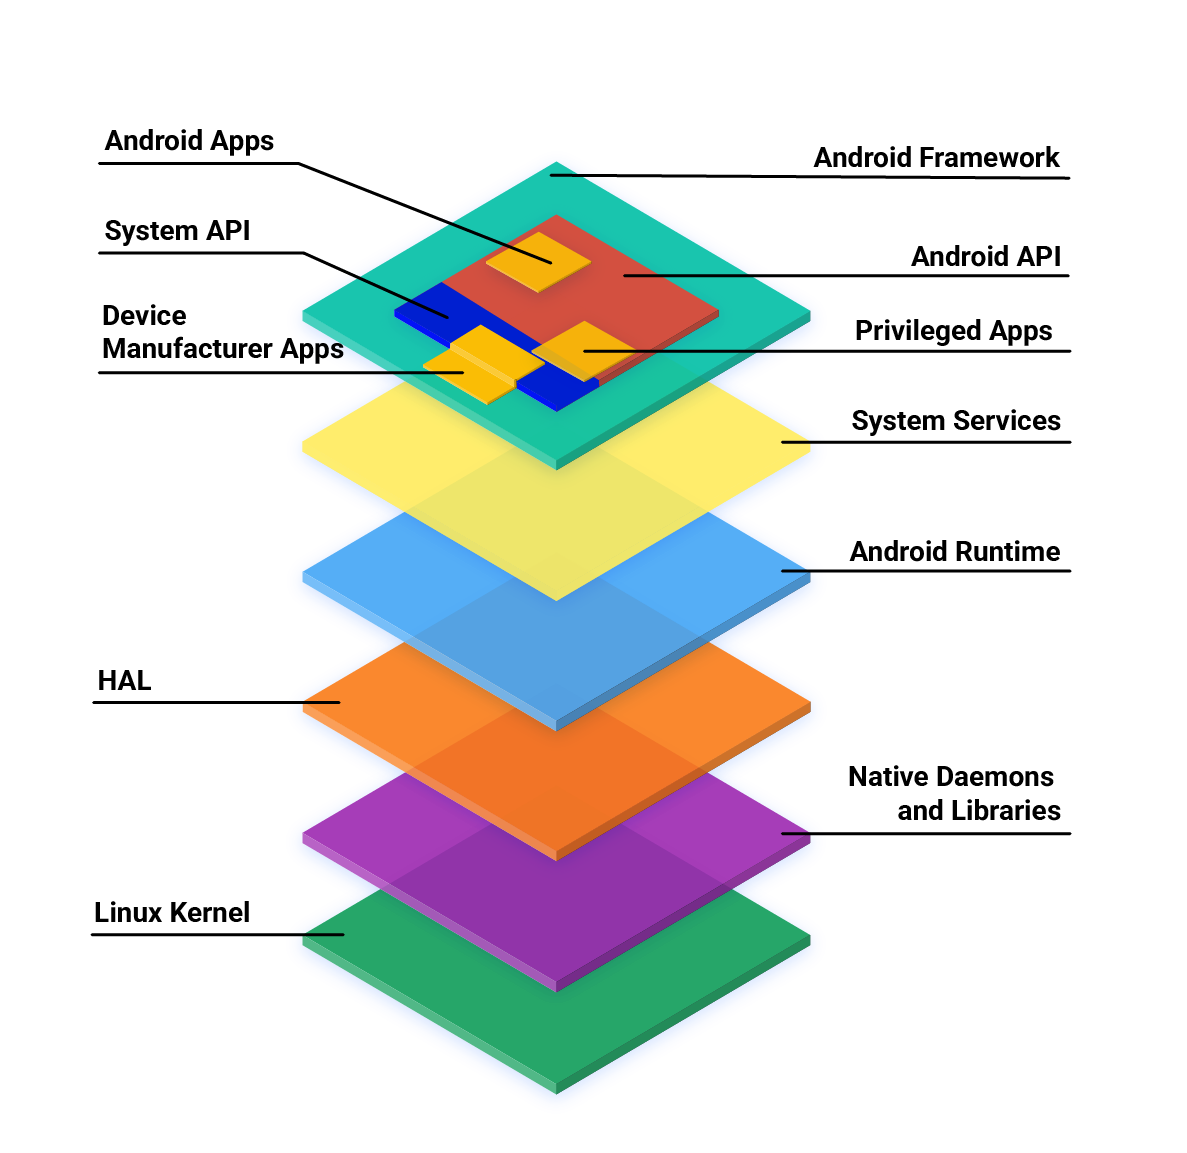
\includegraphics[width=0.8\textwidth]{android_stack.png}
    \caption{AOSP software stack architecture \cite{android-architecture}}
    \label{fig:android_stack}
\end{figure}
\section{Aplicații}
Aplicațiile Android pot fi scrise folosind Kotlin, limbajul de programare Java și limbajele C++. 
Instrumentele SDK Android compilează codul împreună cu orice fișiere de date și resurse într-un APK sau un Android App Bundle.\cite{android-application-fundamentals}

Un pachet Android, care este un fișier de arhivă cu extensia \textit{.apk}, 
conține fișierele unei aplicații Android necesare la rulare și este fișierul pe care dispozitivele cu Android îl folosesc pentru a instala aplicația.\cite{android-application-fundamentals}

Un Android App Bundle, care este un fișier de arhivă cu extensia \textit{.aab}, 
conține fișierele unui proiect de aplicație Android, inclusiv unele metadate suplimentare care nu sunt necesare la rulare. 
Un AAB este un format de publicare și nu poate fi instalat pe dispozitivele Android. 
Generarea și semnarea APK-ului sunt amânate pentru o etapă ulterioară.\cite{android-application-fundamentals}

Fiecare aplicație Android funcționează într-un sandbox de securitate propriu, protejat de următoarele caracteristici de securitate ale Android\cite{android-application-fundamentals}:
\begin{itemize}
    \item Sistemul de operare Android este un sistem Linux multi-utilizator în care fiecare aplicație este un utilizator diferit.
    \item În mod implicit, sistemul atribuie fiecărei aplicații un ID unic de utilizator Linux, care este utilizat doar de sistem și este necunoscut aplicației. Sistemul setează permisiuni pentru toate fișierele dintr-o aplicație astfel încât doar ID-ul de utilizator atribuit acelei aplicații să le poată accesa.
    \item Fiecare proces are propria sa mașină virtuală (VM), astfel încât codul unei aplicații rulează izolat de alte aplicații.
    \item În mod implicit, fiecare aplicație rulează în propriul proces Linux. Sistemul Android pornește procesul atunci când oricare dintre componentele aplicației trebuie să fie executate și închide procesul atunci când nu mai este necesar sau când sistemul trebuie să recupereze memorie pentru alte aplicații.
\end{itemize}

Sistemul Android implementează principiul privilegiului minim (\textit{principle of least privilege}). 
Adică, fiecare aplicație, în mod implicit, are acces doar la componentele de care are nevoie pentru a-și îndeplini funcțiile și nimic mai mult. 
Acest lucru creează un mediu foarte sigur în care o aplicație nu poate accesa părți ale sistemului pentru care nu i s-au acordat permisiuni.\cite{android-application-fundamentals}

Cu toate acestea, există modalități prin care o aplicație poate partaja date cu alte aplicații și prin care o aplicație poate accesa servicii de sistem\cite{android-application-fundamentals}:
\begin{itemize}
    \item Este posibil să se aranjeze ca două aplicații să partajeze același ID de utilizator Linux, caz în care acestea pot accesa fișierele uneia alteia. Pentru a conserva resursele sistemului, aplicațiile cu același ID de utilizator pot, de asemenea, să aranjeze să ruleze în același proces Linux și să partajeze aceeași mașină virtuală (VM). Aplicațiile trebuie, de asemenea, să fie semnate cu același certificat.
    \item O aplicație poate solicita permisiunea de a accesa datele dispozitivului, cum ar fi locația dispozitivului, camera și conexiunea Bluetooth. Utilizatorul trebuie să acorde explicit aceste permisiuni.
\end{itemize}

\subsection{Permisiuni}
Permisiunile aplicațiilor ajută la protejarea confidențialității utilizatorilor\cite{android-permissions} prin restricționarea accesului la următoarele:
\begin{itemize}
    \item Date restricționate, cum ar fi starea sistemului și informațiile de contact ale utilizatorilor
    \item Acțiuni restricționate, cum ar fi conectarea la un dispozitiv împerecheat și înregistrarea audio
\end{itemize}

Tipul fiecărei permisiuni indică domeniul datelor restricționate la care aplicația ta poate avea acces și domeniul acțiunilor restricționate 
pe care aplicația ta le poate efectua atunci când sistemul acordă permisiunea respectivei aplicații.\cite{android-permissions}
Android categorizează permisiunile în diferite tipuri:

\begin{itemize}
    \item \textbf{Install-time} - Oferă aplicației acces limitat la date restricționate sau permit să efectueze acțiuni restricționate care afectează minim sistemul sau alte aplicații.\cite{android-permissions} 
    
    Android include două subtipuri de permisiuni la instalare:
    \begin{itemize}
        \item \textbf{Normale} - Aceste permisiuni permit accesul la date și acțiuni care depășesc sandbox-ul aplicației tale, 
        dar prezintă foarte puțin risc pentru confidențialitatea utilizatorului și funcționarea altor aplicații.\cite{android-permissions}
        \item \textbf{Semnatură (Signature)} - Sistemul acordă o permisiune de semnătură unei aplicații numai atunci când 
        aplicația este semnată cu același certificat ca aplicația sau sistemul de operare care definește permisiunea.\cite{android-permissions}
        
        Aplicațiile care implementează servicii privilegiate, cum ar fi serviciile de completare automată sau VPN, folosesc, de asemenea, permisiuni de semnătură, 
        necesare pentru legarea serviciilor, astfel încât numai sistemul să se poată lega la servicii.\cite{android-permissions}
    \end{itemize}
    \item \textbf{Runtime} - Cunoscute sub numele de permisiuni periculoase, 
    oferă aplicației tale acces suplimentar la date restricționate sau îi permit să efectueze acțiuni restricționate 
    care afectează mai substanțial sistemul și alte aplicații.\cite{android-permissions}

    Multe permisiuni de rulare accesează date private ale utilizatorilor, un tip special de date restricționate care include informații potențial sensibile. 
    Exemple de date private ale utilizatorilor includ locația și informațiile de contact.\cite{android-permissions}

    \item \textbf{Speciale} - Permisiunile speciale corespund unor operațiuni particulare ale aplicațiilor.
    Doar platforma și producătorii originali de echipamente (OEM) pot defini permisiuni speciale. 
    În plus, platforma și producătorii originali de echipamente definesc de obicei permisiuni speciale 
    atunci când doresc să protejeze accesul la acțiuni deosebit de puternice, cum ar fi afișarea unui UI peste alte aplicații.\cite{android-permissions}
\end{itemize}

\subsection{Componente}
Componentele aplicației sunt blocurile esențiale ale unei aplicații Android, 
care reprezintă puncte de intrare prin care sistemul sau un utilizator poate accesa aplicația.\cite{android-application-fundamentals}

Există patru tipuri de componente care pot fi folosite într-o aplicație Android:
\begin{itemize}
    \item \textbf{Activități} - un punct de intrare pentru interacțiunea cu utilizatorul. Reprezintă o singură fereastră cu o interfață de utilizator.\cite{android-application-fundamentals}
    \item \textbf{Servicii} - un punct de intrare general pentru menținerea aplicației în fundal din diverse motive. 
    Este o componentă care rulează în fundal pentru a efectua operațiuni de lungă durată sau pentru a efectua sarcini pentru procesele la distanță. 
    Un serviciu nu furnizează o interfață de utilizator.\cite{android-application-fundamentals}
    \item \textbf{Receptoare de difuzare (Broadcast Receivers)} - o componentă care permite sistemului să livreze evenimente aplicației în afara unui flux normal de utilizator, 
    astfel încât aplicația să poată răspunde anunțurilor de difuzare la nivel de sistem. 
    Deoarece receptoarele de difuzare sunt un alt punct de intrare bine definit în aplicație, 
    sistemul poate livra difuzări chiar și aplicațiilor care nu rulează în prezent.\cite{android-application-fundamentals}
    \item \textbf{Furnizori de conținut (Content Providers)} - o componentă care gestionează un set partajat de date ale aplicației pe care le poți stoca în sistemul de fișiere, 
    într-o bază de date SQLite, pe web sau în orice alt loc de stocare persistentă accesibil aplicației tale. 
    Prin intermediul furnizorului de conținut, alte aplicații pot interoga sau modifica datele, dacă furnizorul de conținut permite acest lucru.\cite{android-application-fundamentals}
\end{itemize}

\subsection{Fișierul manifest}
Înainte ca sistemul Android să poată porni o componentă a aplicației, sistemul trebuie să știe că acea componentă există citind fișierul manifest al aplicației, 
\textit{AndroidManifest.xml}. Aplicația declară toate componentele sale în acest fișier, care se află la rădăcina directorului proiectului aplicației.\cite{android-application-fundamentals}

Pe lângă aceasta, fișierul manifest răspunde de următoarele:
\begin{itemize}
    \item Identifică orice permisiuni de utilizator de care are nevoie aplicația, cum ar fi accesul la internet sau accesul de citire la contactele utilizatorului.
    \item Declară nivelul minim al API-ului necesar aplicației, în funcție de API-urile pe care le folosește aplicația.
    \item Declară caracteristicile hardware și software utilizate sau necesare aplicației, cum ar fi o cameră, servicii Bluetooth sau un ecran multitouch.
    \item Declară bibliotecile API de care aplicația are nevoie pentru a fi legate (altele decât API-urile framework-ului Android).
\end{itemize}

\section{Android Runtime și Dalvik}
\subsection{Bytecode-ul Dalvik}
\subsection{Formatul DEX}
\subsection{Instrucțiunile Dalvik Executable}

\chapter{Soluţia propusă şi metodologia de proiectare/dezvoltare}
\section{Arhitectura sistemului}
\section{Descrierea metodologiei}

\chapter{Implementare}
\section{Tehnologii utilizate}
\section{Descrierea implementării}

\chapter{Utilizare, rezultate experimentale}
\section{Descrierea procesului de testare}
\section{Rezultate experimentale}

\chapter{Concluzii, contribuţii şi direcţii de continuare a dezvoltării}
\section{Concluzii}
\section{Contribuții}
\section{Direcții viitoare}

\addcontentsline{toc}{chapter}{Bibliografie}
\bibliographystyle{plainnat}
\bibliography{bibliography}

% \appendix
% \chapter{Anexe}
% \section{Cod sursă}
% \lstinputlisting[language=Python]{source_code.py}

\end{document}
